% Chapter Template

\chapter{Ensayos y resultados} % Main chapter title
\label{Chapter4} % Change X to a consecutive number; for referencing this chapter elsewhere, use \ref{ChapterX}

En este capítulo se presentan las pruebas realizadas para comprobar el funcionamiento de la plataforma y las diferencias que presenta con respecto a la placa real. Además, se describen las diferentes herramientas que se utilizaron.

%----------------------------------------------------------------------------------------
\section{Banco de pruebas}
%----------------------------------------------------------------------------------------

Para verificar el funcionamiento de la plataforma de emulación se emplearon diversos recursos de software y hardware, que permiten una evaluación completa del funcionamiento de la plataforma, garantizando su confiabilidad y funcionalidad. 

El proceso de verificación incluye también pruebas comparativas entre la plataforma  emulación y la placa física, donde se ejecutaron casos de prueba idénticos en ambos entornos. Esto permite identificar y analizar las diferencias entre el comportamiento real y la del emulador web, además, proporciona información valiosa para mejorar la precisión y fiabilidad de la plataforma web de emulación.

En la tabla \ref{tab:RecursosHardware} se presentan los recursos de hardware empleados en el banco de pruebas.

\begin{table}[h]
	\centering
	\caption[Recursos de hardware utilizados]{Recursos de hardware utilizados.}
	\begin{tabular}{l c}    
		\toprule
		\textbf{Herramienta} & \textbf{Propósito}\\
		\midrule
		Computadora & Acceso a la plataforma de emulación.\\		
		Placa EDU-CIAA-NXP &  Implementación de los ejemplos de la sAPI.\\
		LEDs  &  Pruebas de ejemplo.\\
		Potenciómetro de 10K  &  Pruebas de ejemplo.\\
		Analog Stick  &  Pruebas de ejemplo.\\
		Termistor NTC  &  Pruebas de ejemplo.\\
		Sensor de temp. y hum. DHT11 &  Pruebas de ejemplo.\\
		Display LCD HD44780 &  Pruebas de ejemplo.\\
		Display GLCD ST7920 &  Pruebas de ejemplo.\\
		\bottomrule
		\hline
	\end{tabular}
	\label{tab:RecursosHardware}
\end{table}

Asimismo, se utilizaron herramientas de software para realizar las pruebas
en todos los módulos que componen el sistema. En la tabla \ref{tab:RecursosSoftware} se describe el propósito de estas herramientas.

\hfill \break
\hfill \break
\hfill \break
\hfill \break

\begin{table}[h]
	\centering
	\caption[Recursos de software utilizados]{Recursos de software utilizados.}
	\begin{tabular}{l c}    
		\toprule
		\textbf{Herramienta} & \textbf{Propósito}\\
		\midrule
		Mocha &  Pruebas automatizadas para el frontend.\\		
		Chai &   Pruebas automatizadas para el frontend.\\
		Chrome & Pruebas de la plataforma web.\\
		Firefox & Pruebas de la plataforma web.\\
		Explorer &  Pruebas de la plataforma web. \\
		PostMan \citep{Postman} &  Pruebas de \textit{request} de la plataforma y APIs. \\
		CMocka &  Pruebas automatizadas para el backend. \\
		GCC  & Para la compilación de las pruebas de backend. \\
		Check  & Para la ejecución de las pruebas de backend. \\
		Mocha  &  Pruebas automatizadas para el frontend. \\
		Chai  &  Pruebas automatizadas para el frontend. \\
        Tera Term \citep{TeraTerm} &  Emulador de la terminal serial. \\
		\bottomrule
		\hline
	\end{tabular}
	\label{tab:RecursosSoftware}
\end{table}

%----------------------------------------------------------------------------------------
\section{Pruebas de Unidad} 
\label{subsec:Pruebas de Unidad}  
%----------------------------------------------------------------------------------------

Las pruebas de unidad se centran en evaluar de manera aislada cada función de los archivos de código fuente de la biblioteca C, con el objetivo de que cada unidad de código funcione correctamente y produzca los resultados esperados. 

Como se comenta previamente, para el desarrollo de las pruebas unitarias, se utilizaron \textit{Check} y \textit{CMocka}, que son bibliotecas de pruebas unitarias escritas en lenguaje \textit{C}. \textit{CMocka} proporciona funcionalidades para simular o mockear las funciones y dependencias externas de \textit{emscripten}, lo que posibilita enfocarse en probar exclusivamente los módulos de la biblioteca C.

Además, para compilar las pruebas unitarias con \textit{CMocka} o \textit{Check}, se utiliza el compilador \textit{GCC (GNU Compiler Collection)}. El proceso consiste en compilar los archivos fuente de las pruebas y generar un archivo ejecutable que contiene el resultado del proceso de compilación y enlazado. Los resultados de las pruebas unitarias se muestran en la consola al ejecutar el archivo generado, donde se inica:

\begin{itemize}
	\item El porcentaje de pruebas probadas.
	\item La cantidad de pruebas que aprobaron.
	\item La cantidad de pruebas que fallaron.
	\item Si alguna prueba falla, entonces, indicara el error específico.
	\item Si alguna prueba falla, proporcionará detalles adicionales para identificar el problema.
\end{itemize}

Se desarrollaron estas pruebas y se registraron los resultados en la consola. La figura \ref{fig:PruebasUnidad1} muestra la primera parte de la salida por consola durante la depuración de las pruebas unitarias y la figura \ref{fig:PruebasUnidad2} muestra la segunda parte.

\begin{figure}[ht]
	\centering
	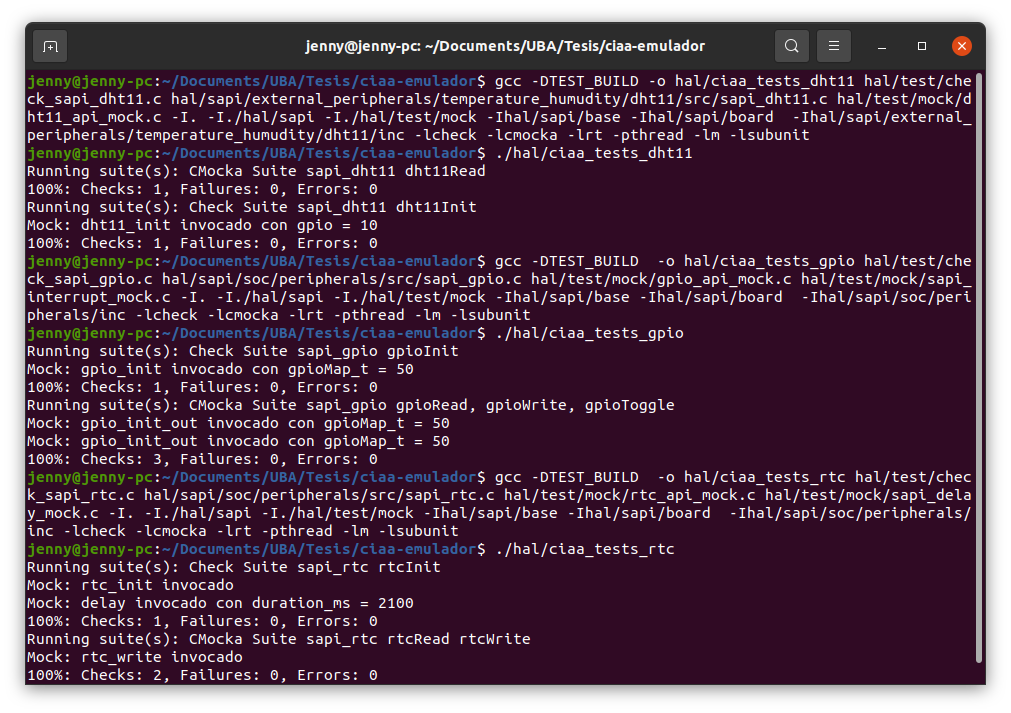
\includegraphics[scale=.27]{./Figures/PruebasUnidad1.png}
	\caption{Primera parte de la salida por consola de las pruebas unitarias con \textit{CMocka} o \textit{Check}.}
	\label{fig:PruebasUnidad1}
\end{figure}

\begin{figure}[ht]
	\centering
	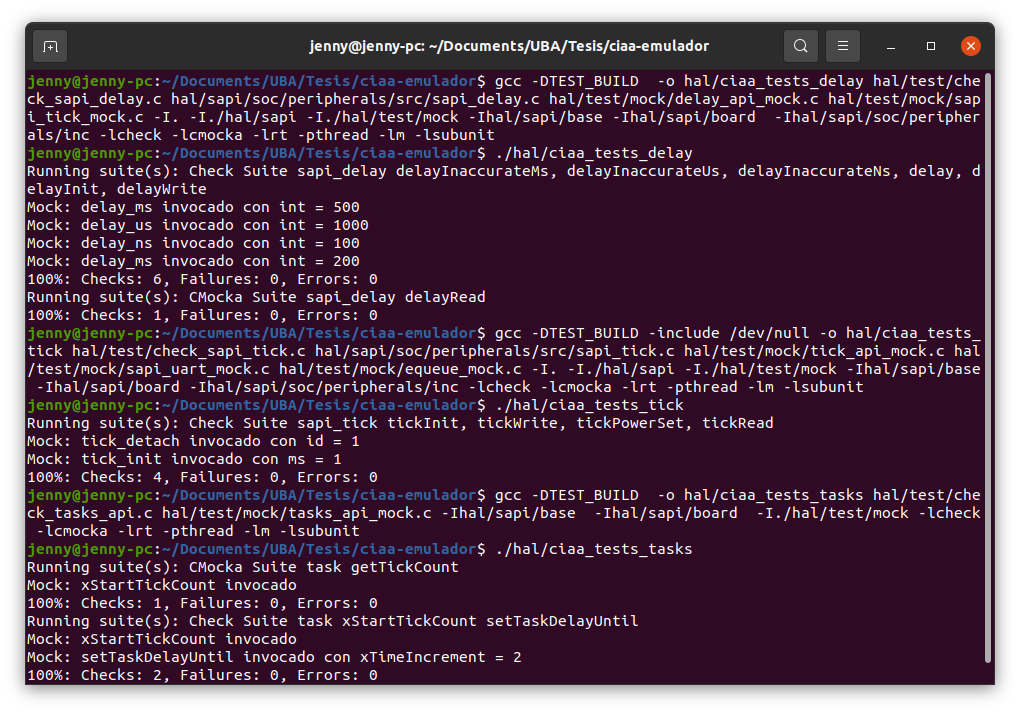
\includegraphics[scale=.27]{./Figures/PruebasUnidad2.png}
	\caption{Segunda parte de la salida por consola de las pruebas unitarias con \textit{CMocka} o \textit{Check}.}
	\label{fig:PruebasUnidad2}
\end{figure}
 

%----------------------------------------------------------------------------------------
\section{Pruebas de Integración} 
\label{subsec:Pruebas de Integración}
%----------------------------------------------------------------------------------------

Las pruebas de integración se centran en evaluar la interacción y comunicación entre diferentes componentes. Además, asegura que trabajen en conjunto sin problemas.

A medida que se fueron desarrollando diferentes módulos y funcionalidades del emulador, las pruebas de integración fueron necesarias para identificar posibles conflictos o incompatibilidades entre los distintos componentes de código del emulador web.

Se identificaron las interacciones entre componentes que fueron relevantes a partir de las pruebas de unidad existentes, como \texttt{sapi\_delay} y \texttt{sapi\_tick}. Luego, se identificaron las dependencias de \textit{Emscripten} y las funciones que se invocan entre las diferentes pruebas de unidad. Desués, se crearon archivos de prueba de integración con escenarios especificos que combinen las interacciones entre los componentes y se utilizaron \textit{mocks} para simular comportamientos de funciones de \textit{Emscripten}.

Al igual que en las pruebas de unidad se utilizo el compilador GCC para compilar. A continuacion la figura \ref{fig:PruebasIntegracion} muestra los resultados por consola de las pruebas de integracion.

\begin{figure}[ht]
	\centering
	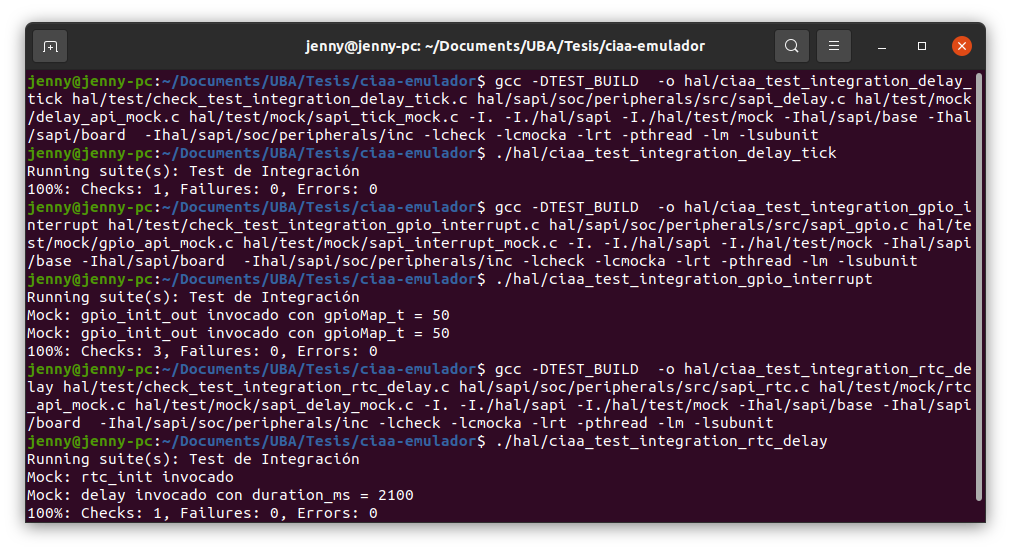
\includegraphics[scale=.35]{./Figures/PruebasIntegracion.png}
	\caption{Depuración de las pruebas de integracion.}
	\label{fig:PruebasIntegracion}
\end{figure}

%----------------------------------------------------------------------------------------
\section{Pruebas de Interfaz de usuario}
\label{sec:Pruebas de Interfaz}
%----------------------------------------------------------------------------------------

Para lograr que la interfaz de la plataforma de emulación cumpla con los requisitos funcionales y logre que los usuarios lo adopten con éxito fue necesario implementar las pruebas de la interfaz de usuario. Por tanto, se implementaron pruebas automatizadas que verifiquen que el funcionamiento sea el correcto, tanto desde la interacción con el usuario así como también con las peticiones hacia el backend.

La implementación de estas pruebas automatizadas permite que se ejecuten de forma rápida y confiable de manera recurrente. 

Para automatizar las pruebas de la interfaz de usuario, se utilizan las bibliotecas \textit{\textbf{Mocha}} y \textit{\textbf{Chai}}, que permiten crear pruebas de interfaz muy completas para el desarrollo en \textit{JavaScript}.

Esto asegura que cada componente de la interfaz funcione correctamente por separado. Incluso, se verifica si el código en el navegador web devuelve los nombres de los módulos correctos, los tipos de parámetros previstos y el tipo de retorno esperado.

La figura \ref{fig:TestVS1} muestra la salida por consola durante la depuración de las pruebas de interfaz con \textit{\textbf{Mocha}}.

\begin{figure}[ht]
	\centering
	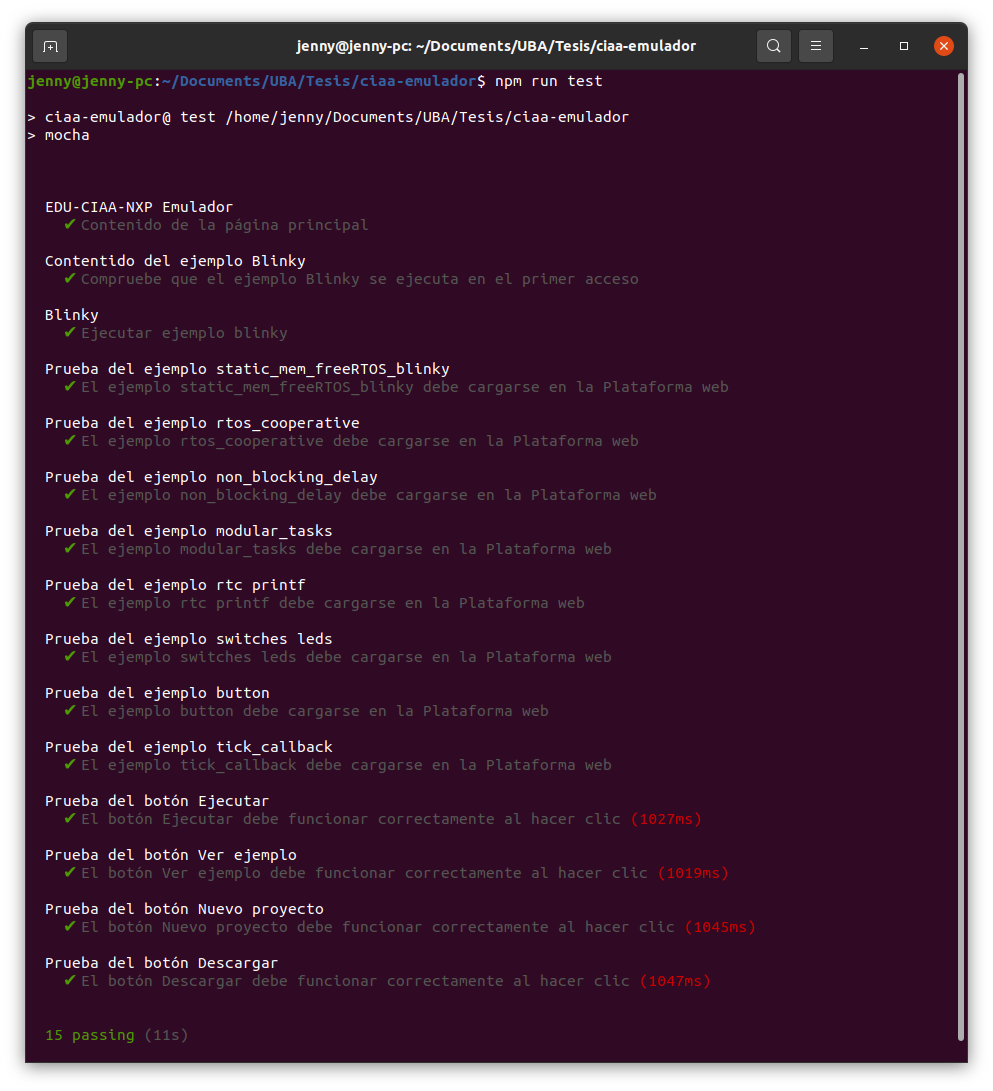
\includegraphics[scale=.29]{./Figures/TestInterfaz.png}
	\caption{Salida por consola durante la depuración de las pruebas de interfaz con \textit{\textbf{Mocha}}.}
	\label{fig:TestVS1}
\end{figure}

%----------------------------------------------------------------------------------------
\section{Integración Continua}
\label{sec:Integracion Continua}
%----------------------------------------------------------------------------------------

Para implementar la integración continua del código se evaluaron dos plataformas:\textit{ GitLab CI} y \textit{Travis CI}. Ambas herramientas, proporcionaron excelentes resultados y demostraron ser igualmente eficaces. Sin embargo, se encontraron algunas diferencias importantes en su configuración y en cómo se presentan las pruebas en cada plataforma.

En el caso de \textit{GitLab CI}, toda la configuración se realizó directamente en la plataforma de \textit{GitLab}, lo que facilitó la integración con el repositorio de la plataforma web y permitió una gestión más centralizada del proceso de \textit{CI/CD}.

Por otro lado, con \textit{Travis CI}, se realizaron configuraciones separadas de \textit{GitHub}. Esto implica un enfoque más descentralizado, lo que puede ser útil si se trabaja en varios proyectos alojados en diferentes repositorios.

Después de evaluar ambas opciones, se decidie utilizar ambas tecnologías, dado que son gratuitas para código abierto, logrando mayor flexibilidad y respaldo en caso de problemas con alguna de estas herramientas.

La experiencia con ambas herramientas fue positiva y permite mejorar la calidad y eficiencia del proceso de desarrollo mediante la automatización de las pruebas unitarias y de integracion, Además de los despliegues continuos.

En ambas plataformas, la información que se muestra en la consola proporciona la siguiente información útil:

\begin{itemize}
	\item Resultado de las pruebas: la consola muestra si las pruebas se ejecutaron con éxito o si hubo fallas en alguna de ellas. 
	
	\item Detalle de los fallos: en el caso de que alguna prueba falle, la consola proporcionará información detallada, como el nombre de la prueba, el nombre del archivo y la línea de código donde ocurrió el error.
	
	\item Información sobre el entorno de prueba: la consola muestra detalles sobre el entorno de prueba utilizado tanto en \textit{Travis CI} como en \textit{GitLab CI}, que incluye la versión del lenguaje de programación, la secuencia de dependencias instaladas y otros detalles de las pruebas.
	
	\item Duración de las pruebas: la consola muestra el tiempo que tardaron todas las pruebas en ejecutarse, de manera que permite identificar las pruebas que deben ser modificadas para optimizar su rendimiento.
	
	\item Logs de ejecución: la consola expone registros detallados de la ejecución de las pruebas, que incluyen mensajes del progreso de las pruebas, información de depuración y los resultados de las mismas.
	
\end{itemize}

La siguiente figura \ref{fig:travis} presenta la consola de \textit{Travis CI}.  

\begin{figure}[ht]
	\centering
	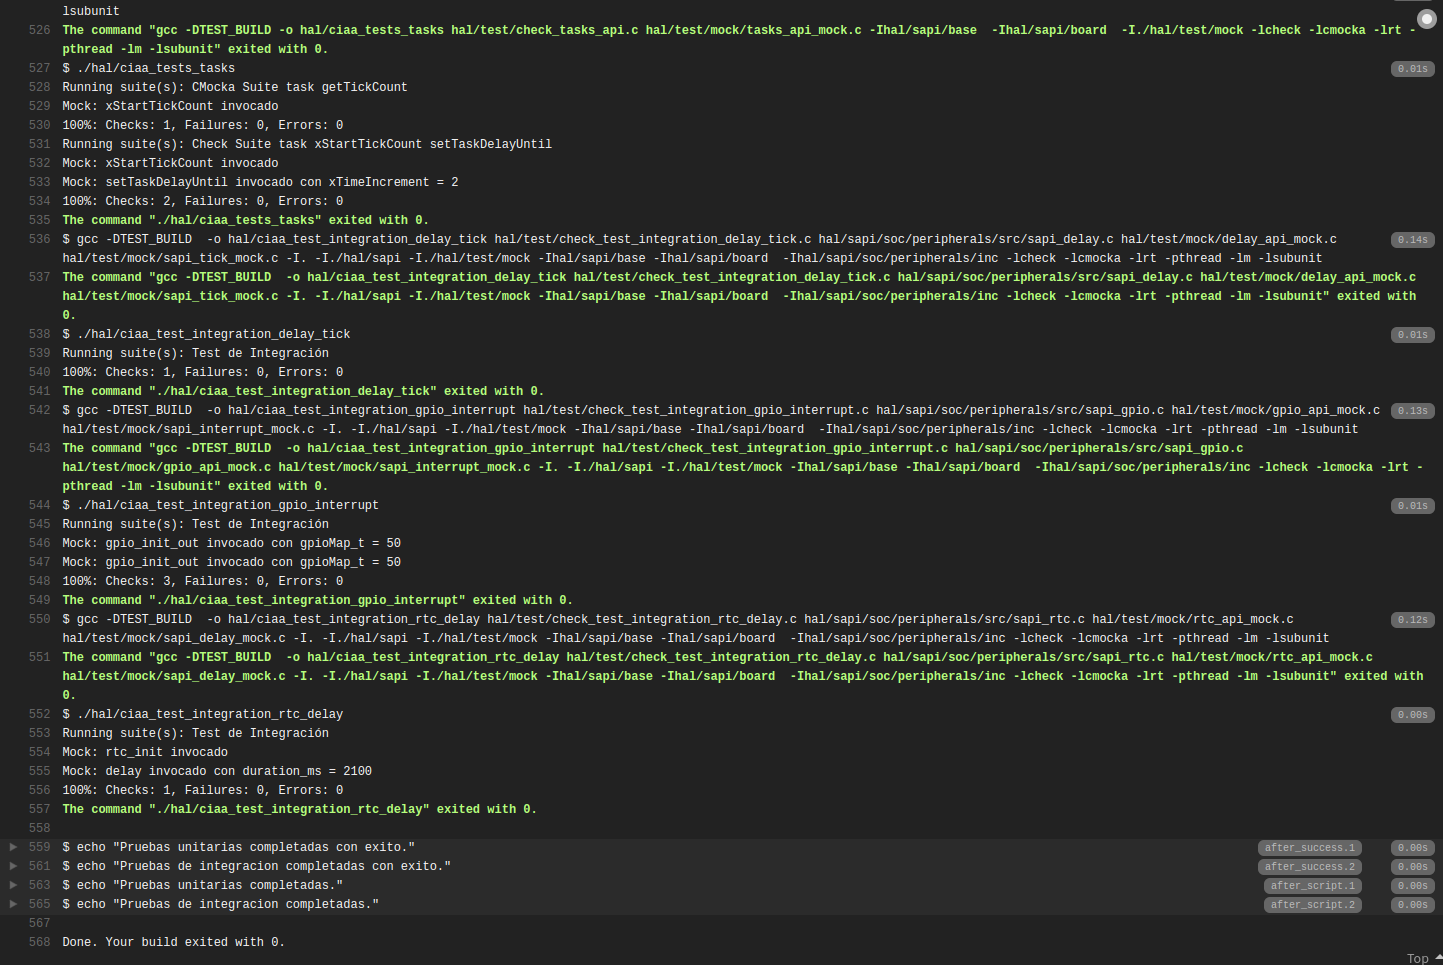
\includegraphics[scale=.35]{./Figures/travis.png}
	\caption{Información de las pruebas que se ejecutaron en \textit{Travis CI}.}
	\label{fig:travis}
\end{figure}

La figura \ref{fig:gitLab} presenta la consola de \textit{GitLab CI}.  

\begin{figure}[ht]
	\centering
	\includegraphics[scale=.40]{./Figures/gitLab.png}
	\caption{Información de las pruebas que se ejecutaron en \textit{GitLab CI}.}
	\label{fig:gitLab}
\end{figure}

\hfill \break
\hfill \break
\hfill \break
\hfill \break
\hfill \break

%------------------------------
\subsection{Prueba de acceso}    

Para verificar y validar el acceso mediante solicitudes HTTP al servidor donde se encuentra publicado \textit{EmuCIAA}, se utiliza la herramienta Postman.

Antes de comenzar con el ensayo, se crea un caso de prueba con el propósito de ser una guía estructurada y documentada para verificar si el acceso al servidor funciona como se espera.

\textit{\textbf{ID Caso de prueba: CP01}}

Descripción: la primera vez que el usuario ingresa a la plataforma de emulación se muestra en ejecución el ejemplo predeterminado \textit{Blinky}.

Pre-condición: 
\begin{itemize}
    \item La computadora del usuario tiene conexión a internet y un navegador web instalado.
\end{itemize}

Flujo principal:
\begin{itemize}
    \item El usuario ingresa al entorno web de la plataforma \textit{EmuCIAA}.
\end{itemize}

Post condiciones:
\begin{itemize}
    \item ÉXITO: la plataforma muestra el ejemplo \textit{\textbf{blinky}} en ejecución, encendiendo y apagando el \textit{LEDB}.
    \item FALLA: La plataforma no muestra ningún ejemplo predeterminado en ejecución.
\end{itemize}

Resumen del Test:
\begin{itemize}
    \item Después de acceder a la plataforma mediante los navegadores web Chrome, Firefox y Explorer se comprobó que se muestra en ejecución el ejemplo \textit{\textbf{blinky}}.
    \item Se realizó la prueba de HTTP \textit{requests} por medio de la utilización de la herramienta \textit{\textbf{Postman}} que luego de acceder a la dirección del servidor donde se encuentra la plataforma, devolvió en formato \textit{\textbf{JSON}} la respuesta del servidor.
\end{itemize}

La figura \ref{fig:PlataformaEmuladorBlinky} muestra la plataforma de emulación ejecutando el ejemplo predeterminado \textit{\textbf{blinky}}.

\begin{figure}[ht]
	\centering
	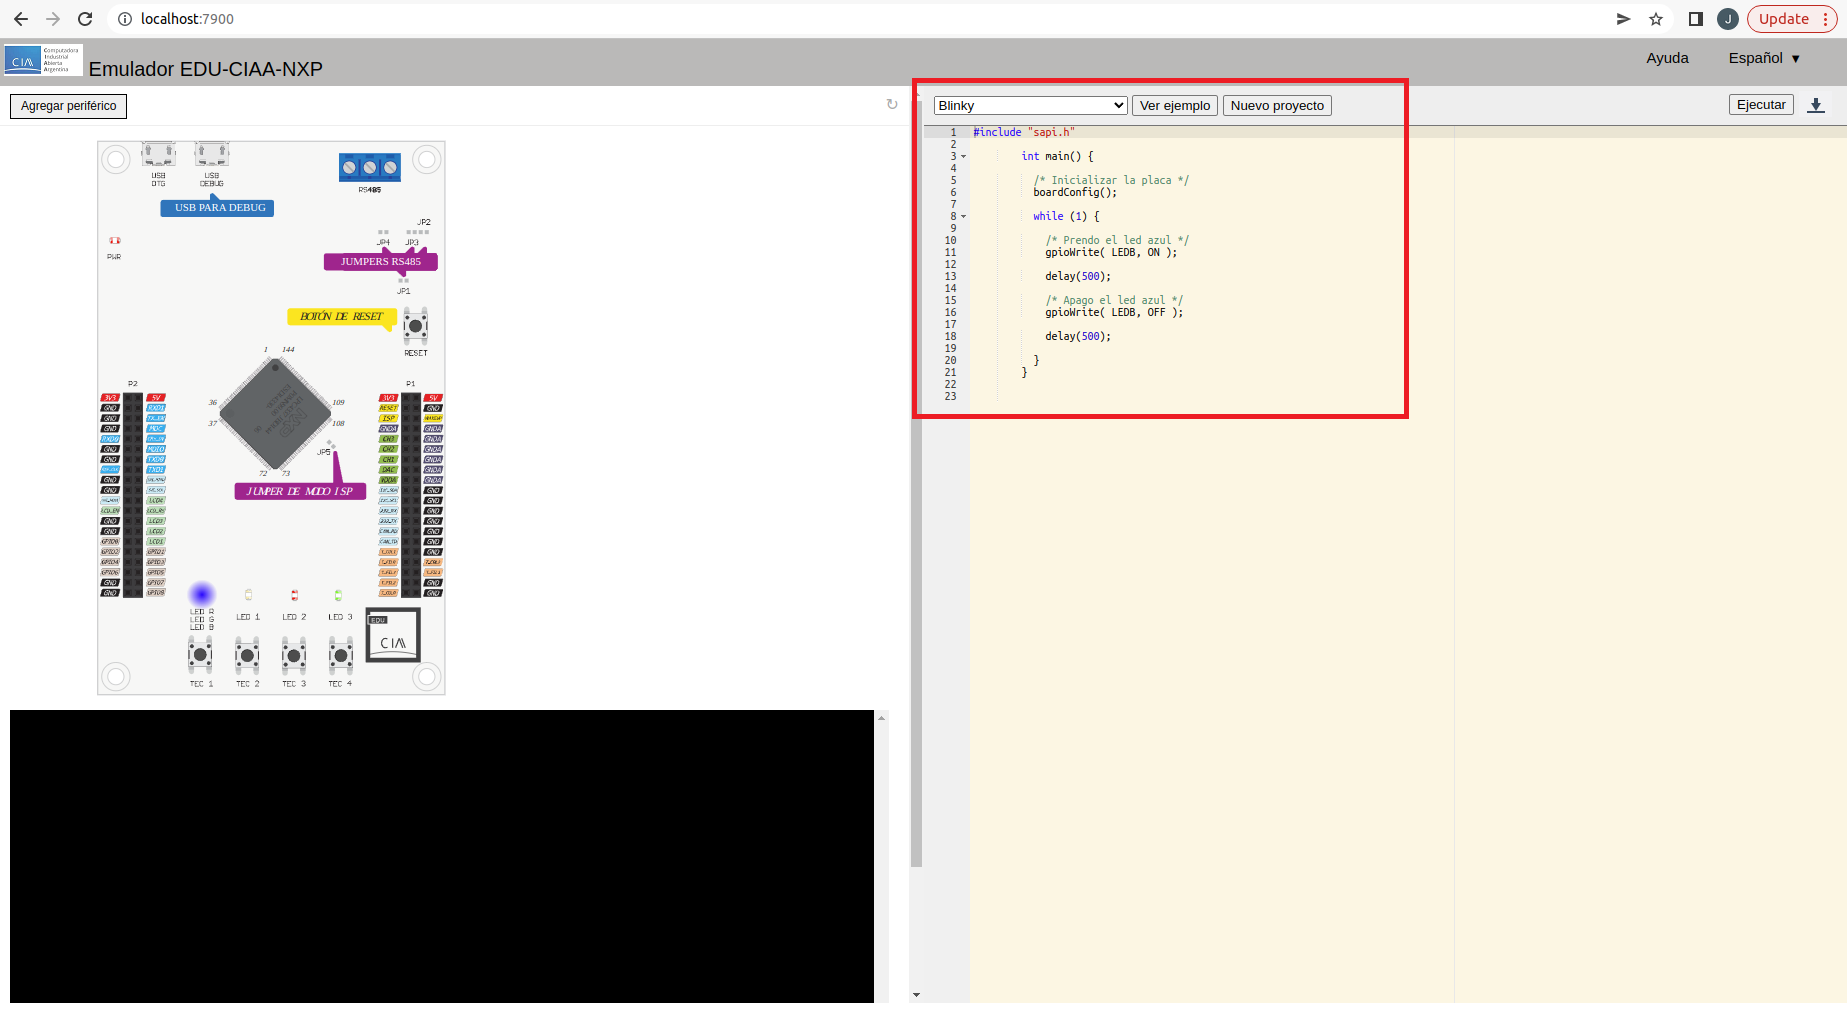
\includegraphics[scale=.21]{./Figures/PlataformaEmuladorBlinky.png}
	\caption{Prueba plataforma emulador ejecutando el ejemplo \textit{\textbf{Blinky}}.}
	\label{fig:PlataformaEmuladorBlinky}
\end{figure}

\textit{\textbf{Postman}} es una aplicación que permite realizar pruebas de API. La herramienta permite realizar pruebas \textit{\textbf{HTTP requests}} y acceder al servidor de la plataforma de emulación. Se obtiene la respuesta en diferentes formatos como \textit{\textbf{JSON}}, \textit{\textbf{XML}}, \textit{\textbf{HTML}} y \textit{\textbf{Text}}.

En la figura \ref{fig:PostmanBlinky2} se muestra la petición y respuesta de acceso a la plataforma por medio de la herramienta \textit{\textbf{Postman}}.

\hfill \break
\hfill \break
\hfill \break
\hfill \break
\hfill \break
\hfill \break
\hfill \break
\hfill \break
\hfill \break
\hfill \break

\begin{figure}[ht]
	\centering
	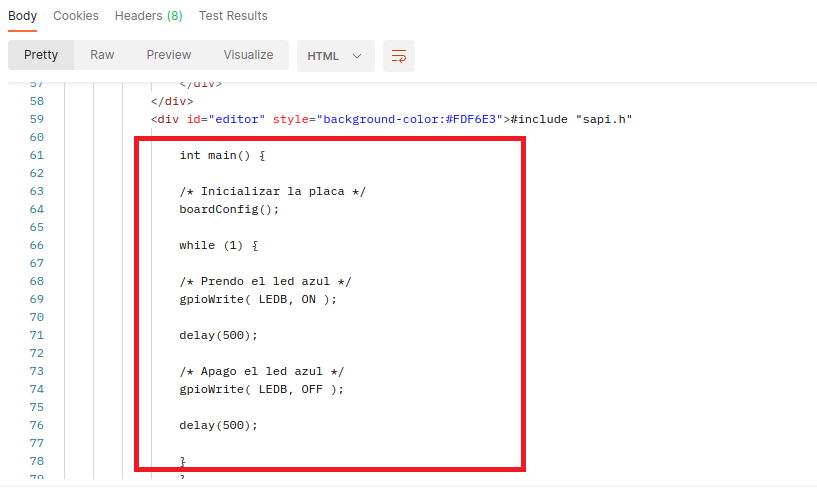
\includegraphics[scale=.40]{./Figures/PostmanBlinky2.png}
	\caption{Respuesta del servidor.}
	\label{fig:PostmanBlinky2}
\end{figure}

%----------------------------------------------------------------------------------------
\section{Pruebas de funcionamiento}  
\label{sec:Pruebas de funcionamiento}
%----------------------------------------------------------------------------------------

Para evaluar, verificar el comportamiento y desempeño de la EDU-CIAA-NXP en el entorno web, se realizan pruebas funcionales con cada uno de los ejemplos contenidos en la plataforma, que cubren la totalidad de periféricos desarrollados.

A modo de ejemplo, a continuación se exponen las pruebas funcionales con uno de los periféricos internos, en este caso, es el RTC, y las pruebas un periférico externo DHT11.

También, se realiza una prueba del ejemplo \textit{tick\_hook}, pero creando un programa utilizando el botón \textquotedbl Nuevo proyecto\textquotedbl. Este ejemplo se utiliza para mostrar las diferencias de tiempo de ejecución entre la plataforma web y la placa física EDU-CIAA-NXP.

%--------------------------------------
\subsection{ Prueba del ejemplo \textit{\textbf{rtc\_printf}}}

%--------------
\subsubsection{Ensayo en \textit{EmuCIAA}} 

Para el ensayo en la plataforma de emulación web se plantea el siguiente caso de prueba:

\textit{\textbf{ID Caso de prueba: CP02}}

Descripción: la plataforma de emulación permite al usuario ejecutar el ejemplo \textit{\textbf{rtc\_printf}}.

Pre-condición: 
\begin{itemize}
    \item La computadora del usuario tiene conexión a internet y un navegador web instalado.
\end{itemize}

Flujo principal:
\begin{enumerate}
	\item El usuario ingresa al entorno web de la plataforma de emulación para la placa EDU-CIAA-NXP.
	\item El usuario selecciona desde la lista desplegable de ejemplos, el ejemplo \textit{\textbf{rtc\_printf}}.
	\item La plataforma muestra en pantalla al usuario el código que corresponde al ejemplo \textit{\textbf{rtc\_printf}}.
	\item El usuario hace click en el botón \textquotedbl Ejecutar\textquotedbl.
	\item La plataforma muestra en la consola integrada la salida la UART, enviando los valores del RTC.
	\item El usuario realiza la descarga del ejemplo \textit{\textbf{rtc\_printf.c}} al hacer click en el botón de descarga, ubicado en el área de codificación.
\end{enumerate}

Post condiciones:
\begin{itemize}
	\item ÉXITO: la plataforma muestra en ejecución el ejemplo \textit{\textbf{rtc\_printf}} al actualizar la salida por consola del envío por UART.
	\item FALLA: La plataforma no muestra al usuario ningún cambio en la consola.
\end{itemize}

Luego de completar el caso de uso CP02, se obtuvo el siguiente resultado: 

\begin{itemize}
	\item ÉXITO: la plataforma muestra en ejecución el ejemplo \textit{\textbf{rtc\_printf}}.
\end{itemize}

La figura \ref{fig:rtcprintf} muestra en la consola integrada la salida del ensayo. 

\begin{figure}[ht]
	\centering
	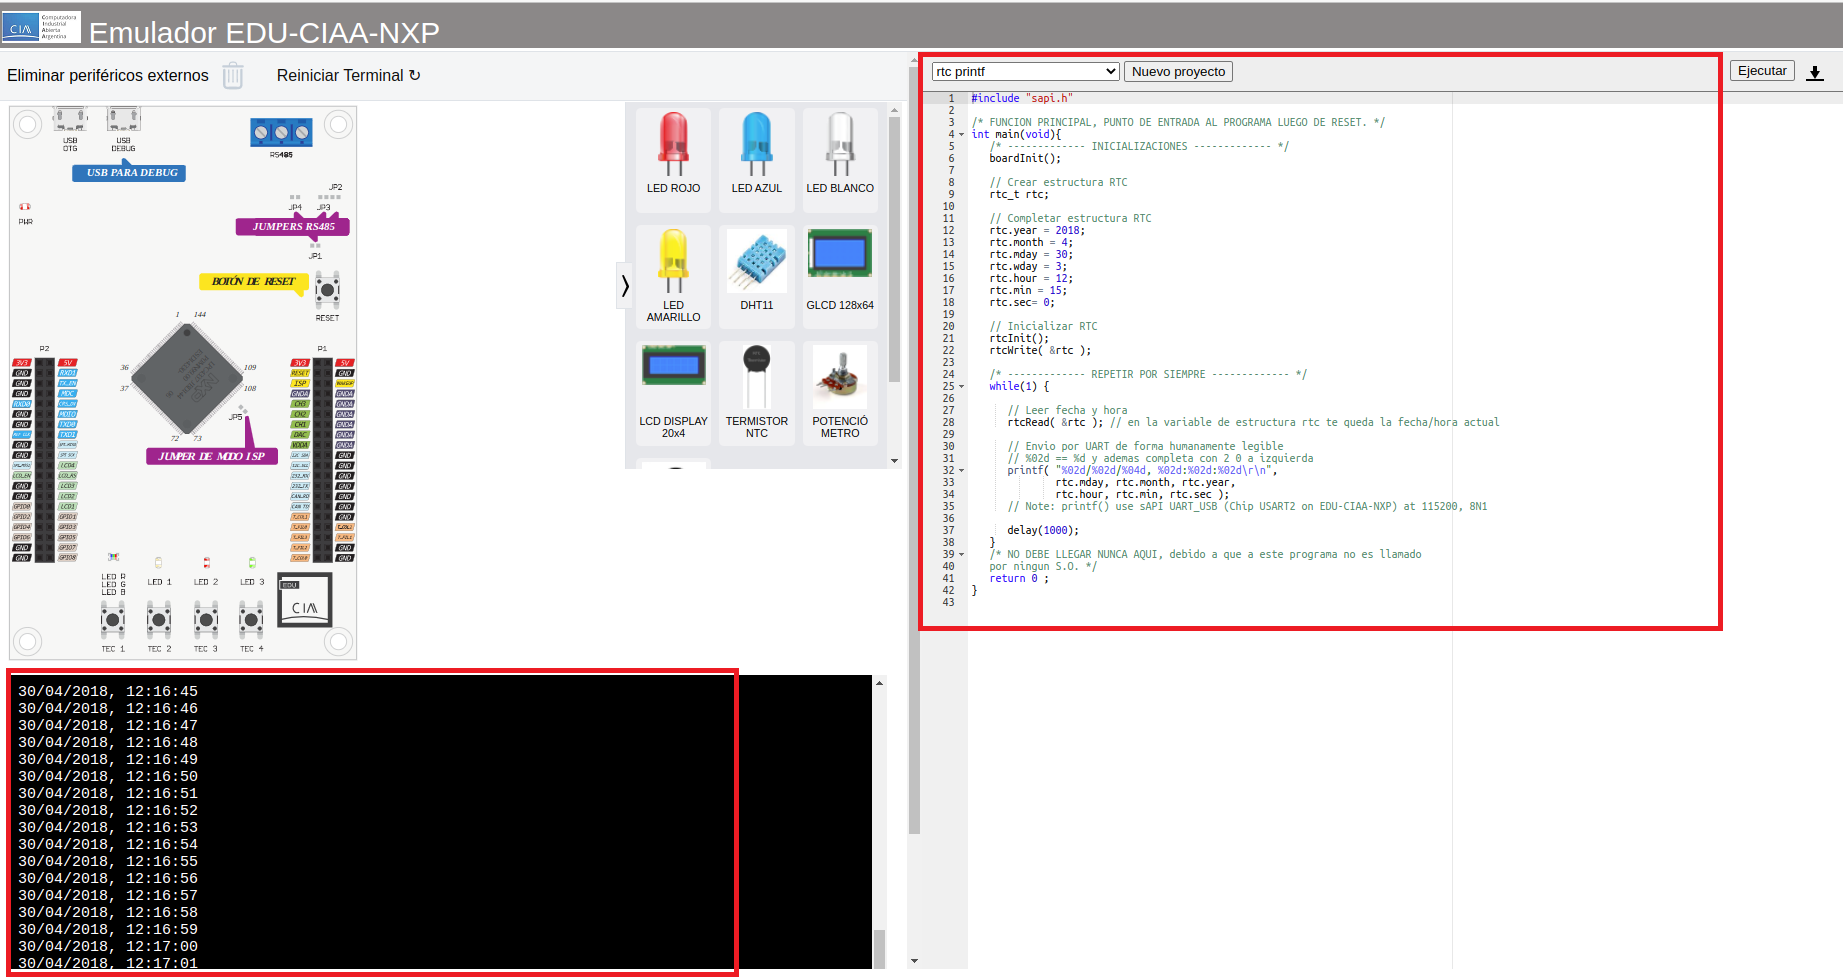
\includegraphics[scale=.21]{./Figures/rtcprintf.png}
	\caption{Salida por consola del ensayo \textit{\textbf{rtc printf}}.}
	\label{fig:rtcprintf}
\end{figure}

%----------------------
\subsubsection{Ensayo en la placa física EDU-CIAA-NXP} 

Primeramente, dentro de la herramienta de desarrollo \textit{eclipse} se importa el archivo \textquotedbl rtc\_printf.c\textquotedbl{} generado por la plataforma web, luego, se realiza las configuraciones necesarias para compilar el proyecto. 

La figura \ref{fig:rtcprintfEclipse} expone el ejemplo \textit{\textbf{rtc\_printf}} importado en \textit{eclipse}: 

\begin{figure}[ht]
	\centering
	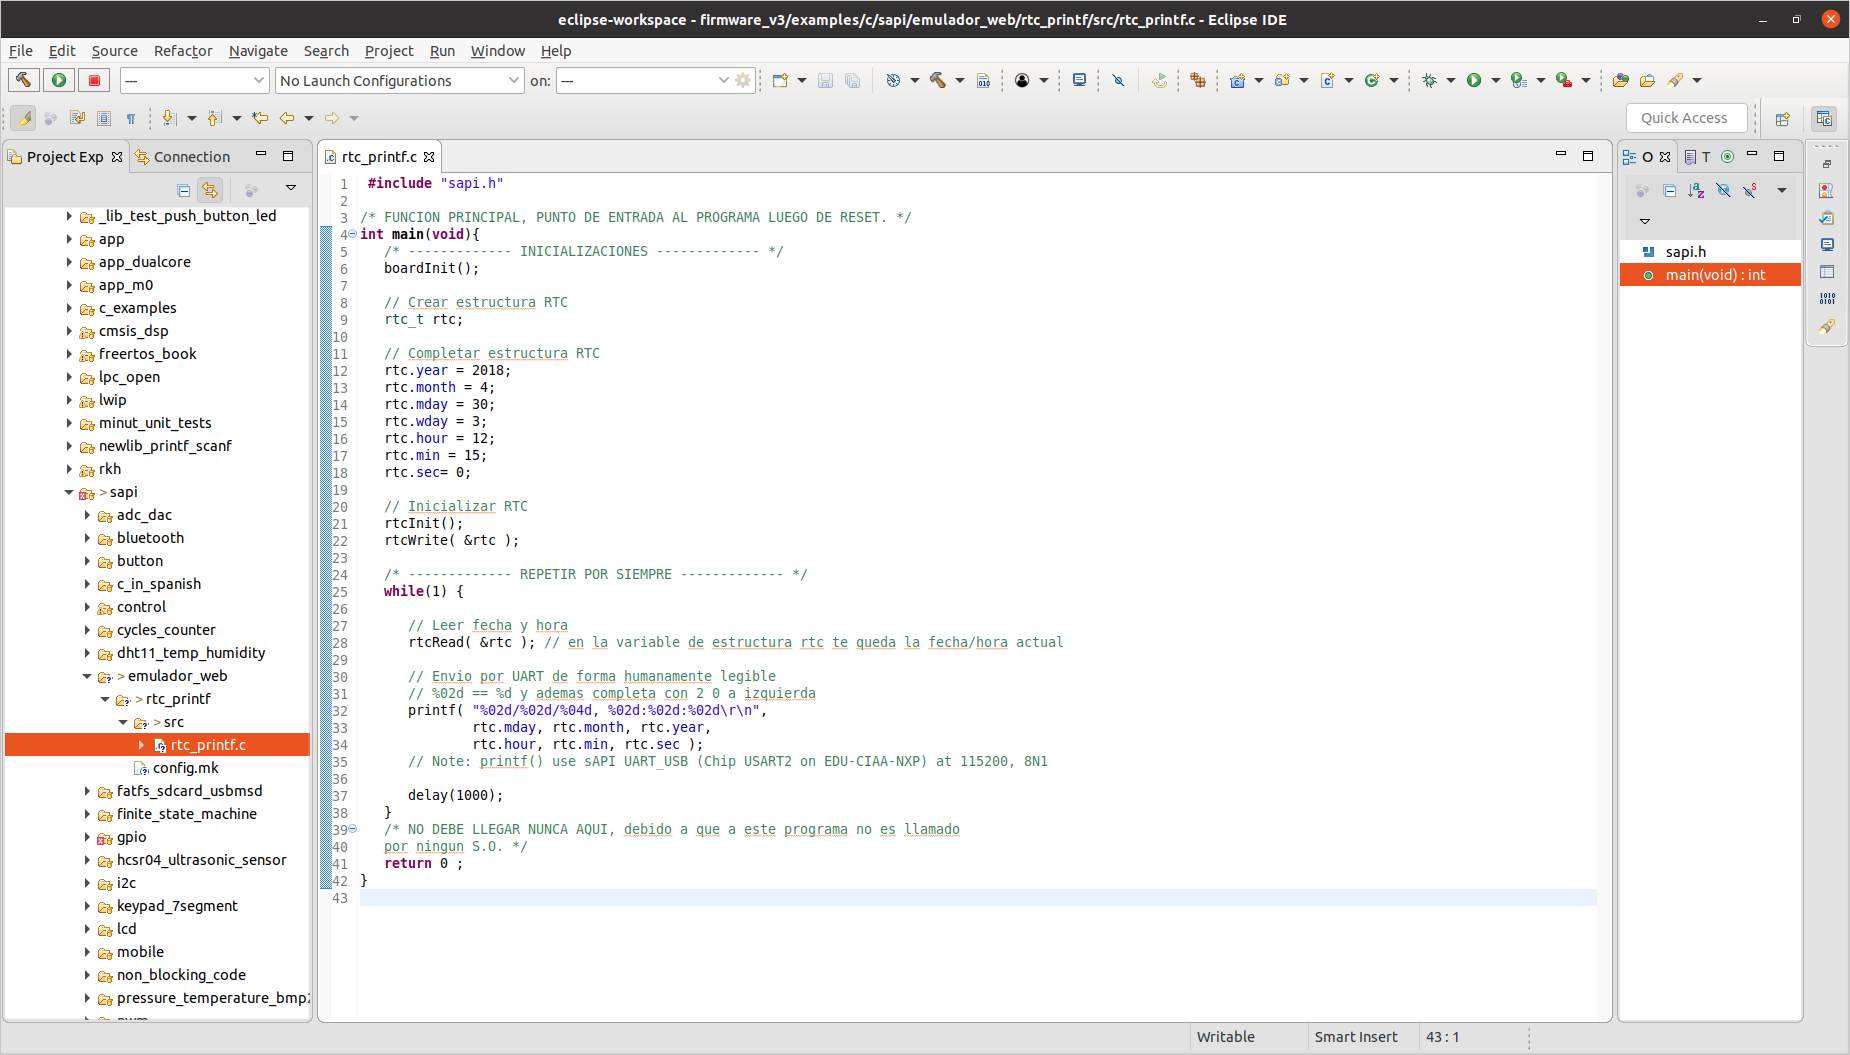
\includegraphics[scale=.20]{./Figures/rtcprintfEclipse.png}
	\caption{Ejemplo \textit{\textbf{rtc printf}} importado en \textit{eclipse}.}
	\label{fig:rtcprintfEclipse}
\end{figure}

\hfill \break

Finalmente, se ejecuta el mismo ejemplo en la placa física EDU-CIAA-NXP y se obtiene por consola la siguiente salida que se muestra en la figura \ref{fig:rtcprintfPlaca}:

\begin{figure}[ht]
	\centering
	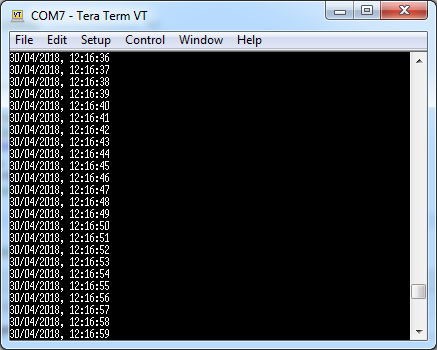
\includegraphics[scale=.90]{./Figures/rtcprintfPlaca.png}
	\caption{Salida de la terminal COM7 -Tera Term VT.}
	\label{fig:rtcprintfPlaca}
\end{figure}

Resumen de la prueba Exitosa:
\begin{itemize}
	\item Después de seguir los pasos del flujo principal del caso de prueba, se comprueba que se muestra en ejecución el ejemplo \textit{\textbf{rtc\_printf}}.
	\item El ensayo en la placa física EDU-CIAA-NXP con el mismo ejemplo, obtuvo la misma salida por consola de la plataforma web.
\end{itemize}


%------------------------------------
\subsection{Prueba del ejemplo \textit{\textbf{dht11}} }

%--------------
\subsubsection{Ensayo en \textit{EmuCIAA}} 

Para el ensayo en la plataforma de emulación web se elabora :

\textit{\textbf{ID Caso de prueba: CP03}}

Descripción: la plataforma de emulación permite al usuario ejecutar el ejemplo \textit{\textbf{dht11}}.

Pre-condición: 
\begin{itemize}
	\item La computadora del usuario tiene conexión a internet y un navegador web instalado.
\end{itemize}

Flujo principal:
\begin{enumerate}
	\item El usuario ingresa al entorno web de la plataforma de emulación para la placa EDU-CIAA-NXP.
	\item El usuario selecciona desde la lista desplegable jerárquica el ejemplo \textit{\textbf{dht11}}.
	\item La plataforma web realiza las siguientes acciones:
	 
	\begin{itemize}
	    \item muestra al usuario el código  del ejemplo \textit{\textbf{dht11}} dentro del área de codificación.
	    \item carga el periférico virtual de manera automática dentro del área de ensamblado y muestra las conexiones a los pines configurados por defecto, los cuales son: \textquotedbl VCC=3V3\textquotedbl, \textquotedbl DATA=GPIO1\textquotedbl y \textquotedbl GND=GND\textquotedbl{}.
	    \item muestra seleccionado la opción por defecto \textquotedbl Obtener datos de servidor climático local.\textquotedbl
	    \item actualiza los termómetros gráficos que corresponden a la temperatura y a la humedad con los datos obtenidos del servidor climático cercano a la ubicación del usuario.
	\end{itemize}

	\item El usuario hace \textit{click} en el botón \textquotedbl Ejecutar\textquotedbl.
	\item La plataforma muestra en la consola integrada la salida de la temperatura y humedad con los valores enviados desde la central meteorológica en línea.
	\item El usuario realiza la descarga del ejemplo \textit{\textbf{dht11}} al hacer \textit{click} en el botón de descarga, ubicado en el área de codificación.
\end{enumerate}

Flujo alternativo:
\begin{enumerate}
    \setcounter{enumi}{3}
	\item El usuario hace \textit{click} en la opción \textquotedbl Establecer Temperatura y Humedad manualmente (haga click y arrastre sobre los indicadores).\textquotedbl
	\item La plataforma deselecciona la opción \textquotedbl Obtener datos de servidor climático local.\textquotedbl
    \item El usuario comienza a manipular los indicadores gráficos haciendo \textit{click} sobre mismos, que corresponden a la temperatura y a la humedad.
    \item La plataforma actualiza los indicadores gráficos con los datos generados por el usuario.

	\item El usuario hace \textit{click} en el botón \textquotedbl Ejecutar\textquotedbl.
	
	\item La plataforma muestra en la consola integrada la salida de la temperatura y humedad según la selección de obtención de datos.
	
	\item El usuario realiza la descarga del ejemplo \textit{\textbf{dht11}} al hacer \textit{click} en el botón de descarga, ubicado en el área de codificación.
\end{enumerate}

Post condiciones:
\begin{itemize}
	\item ÉXITO: la plataforma debe cumplir con todas las siguientes condiciones de éxito:
	
		\begin{itemize}
	    \item  carga automáticamente el periférico virtual dentro del área de ensamblado y las conexiones configuradas por defecto.
	    
	    \item actualiza los indicadores gráficos de temperatura y humedad, que  corresponden a la elección de obtención de datos.

	    \item muestra en ejecución el ejemplo \textit{\textbf{dht11}} y según la elección de obtención de datos, actualiza la salida de temperatura y humedad en la consola integrada.
	    \end{itemize}
	
	\item FALLA: la plataforma no cumple con alguna de las condiciones de éxito descriptas.
\end{itemize}

Luego de completar el caso de uso CP02 con: flujo principal y flujo alternativo, se obtiene el siguiente resultado: 

\begin{itemize}
	\item ÉXITO: la plataforma cumple con todas las condiciones de éxito para el ejemplo \textit{\textbf{dht11}}.
\end{itemize}

La figura \ref{fig:RespuestaEmulador_DHT11_1} muestra la consola con los datos de temperatura y humedad del ejemplo \textit{\textbf{dht11}} con la opción \textquotedbl Obtener datos de servidor climático local.\textquotedbl

\begin{figure}[ht]
	\centering
	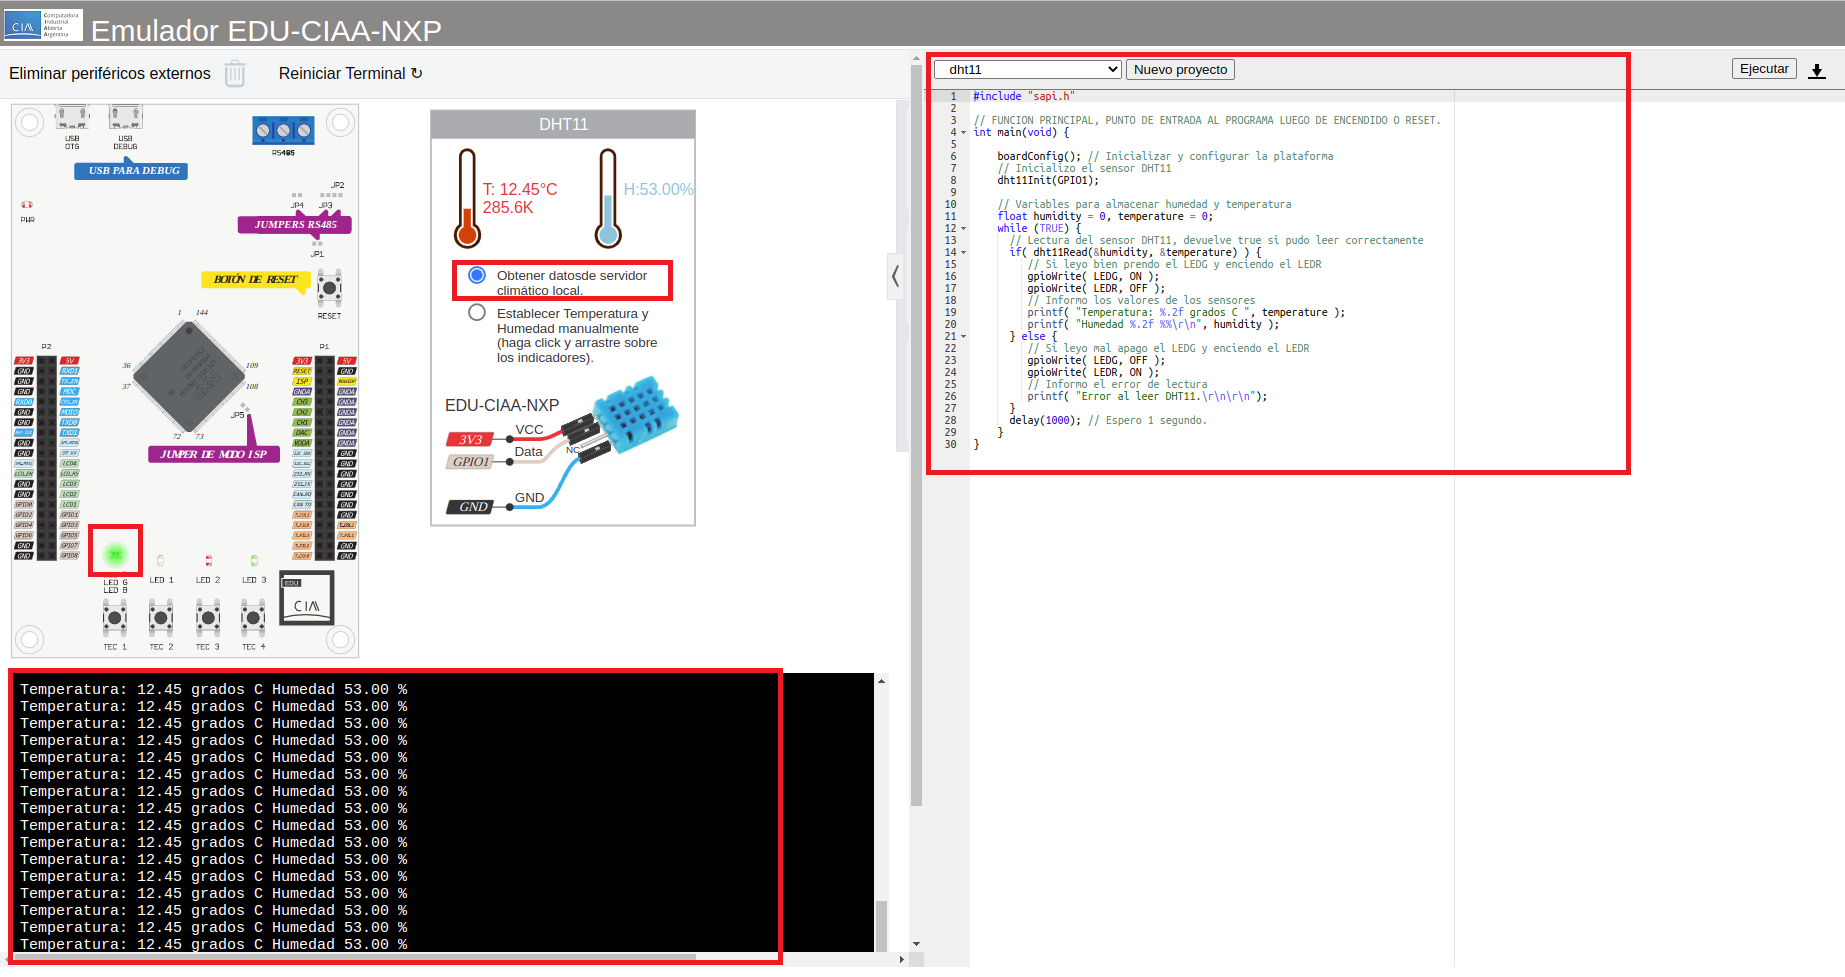
\includegraphics[scale=.20]{./Figures/dht11Opcion1.png}
	\caption{Resultado del  CP02 con la opción \textquotedbl Obtener datos de servidor climático local.\textquotedbl}
	\label{fig:RespuestaEmulador_DHT11_1}
\end{figure}

La figura \ref{fig:RespuestaEmulador_DHT11_2} muestra la consola con los datos de temperatura y humedad del ejemplo \textit{\textbf{dht11}} con la opción \textquotedbl Establecer Temperatura y Humedad manualmente(haga click y arrastre sobre los indicadores).\textquotedbl

\begin{figure}[ht]
	\centering
	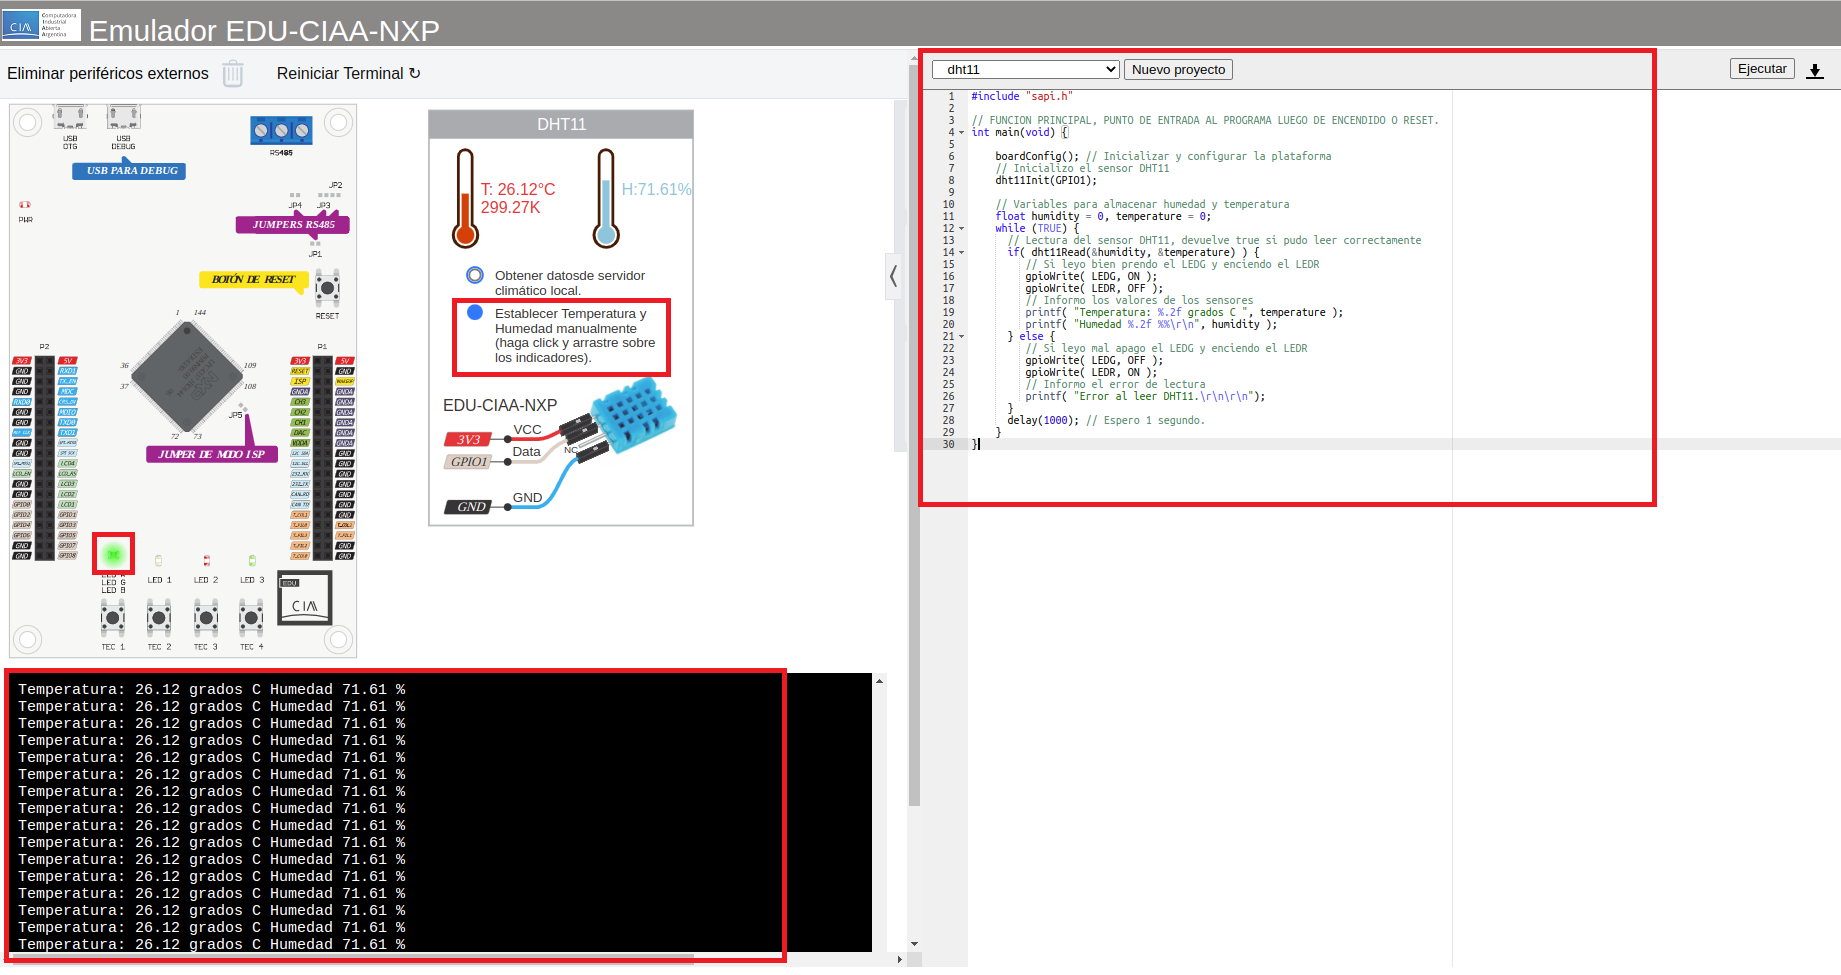
\includegraphics[scale=.20]{./Figures/dht11Opcion2.png}
	\caption{Resultado del CP02 con la opción \textquotedbl Establecer Temperatura y Humedad manualmente(haga click y arrastre sobre los indicadores).\textquotedbl}
	\label{fig:RespuestaEmulador_DHT11_2}
\end{figure}

Para verificar que la plataforma obtuvo los datos de temperatura/humedad de la API de meteorología \textit{\textbf{openweathermap}} se hicieron pruebas de \textit{request} con la herramienta \textit{Postman}.

En la figura \ref{fig:RespuestaPostMan1} se observa que la petición de datos de temperatura/humedad recibe como parámetro la ciudad que se quiere consultar.

\begin{figure}[ht]
	\centering
	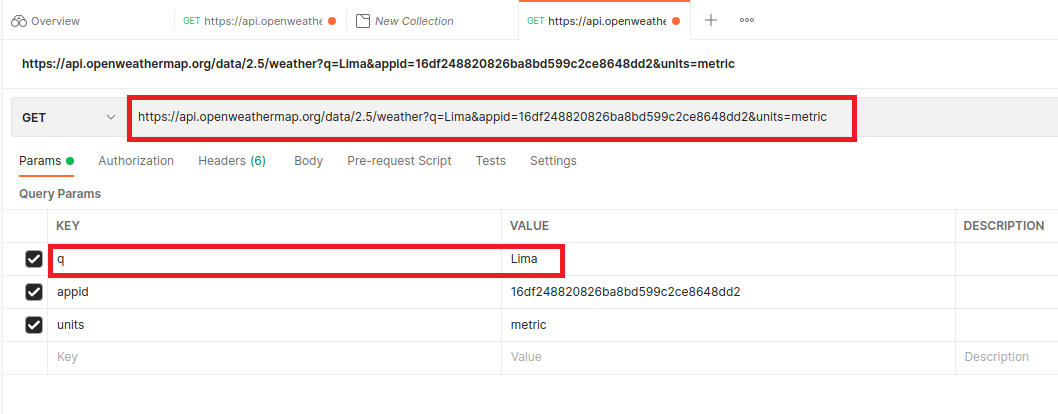
\includegraphics[scale=.30]{./Figures/RespuestaPostMan1.png}
	\caption{Petición de datos de temperatura/humedad.}
	\label{fig:RespuestaPostMan1}
\end{figure}

En este paso se verifica que la respuesta de la petición de datos de temperatura/humedad al API \textit{\textbf{openweathermap}} coincide con lo que se observa en la terminal de la plataforma de emulación.

%----------------------
\subsubsection{Ensayo en la placa física EDU-CIAA-NXP} 

Este ensayo tiene como objetivo identificar las diferencias entre los resultados reales producidos por la placa física EDU-CIAA-NXP y los resultados esperados en la plataforma de emulación.

El primer paso fue conectar el componente DHT11 a la placa EDU-CIAA-NXP. Luego, se procede a importar el archivo generado por la plataforma web \newline\textquotedbl dht11\_temp\_humidity.c\textquotedbl{} y compilarlo dentro de la herramienta 
\textit{eclipse}. Luego, se descarga a la placa física EDU-CIAA-NXP.

En la figura \ref{fig:TestHardware} se muestra la ejecución del ensayo en la plataforma EDU-CIAA-NXP.

\begin{figure}[ht]
	\centering
	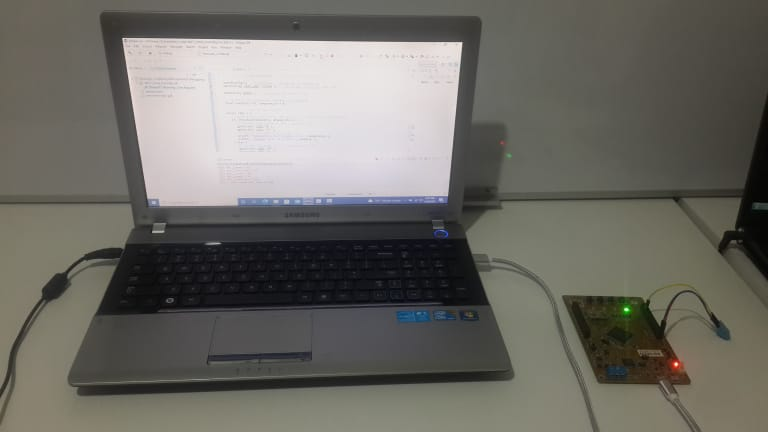
\includegraphics[scale=.45]{./Figures/TestHardware.jpeg}
	\caption{Ensayo en la plataforma EDU-CIAA-NXP del ejemplo \textit{\textbf{dht11}}.}
	\label{fig:TestHardware}
\end{figure}

La figura \ref{fig:TestEclipse} muestra el código del ejemplo \textit{\textbf{dht11}} en la herramienta \textit{eclipse} de la PC de prueba.

\begin{figure}[ht]
	\centering
	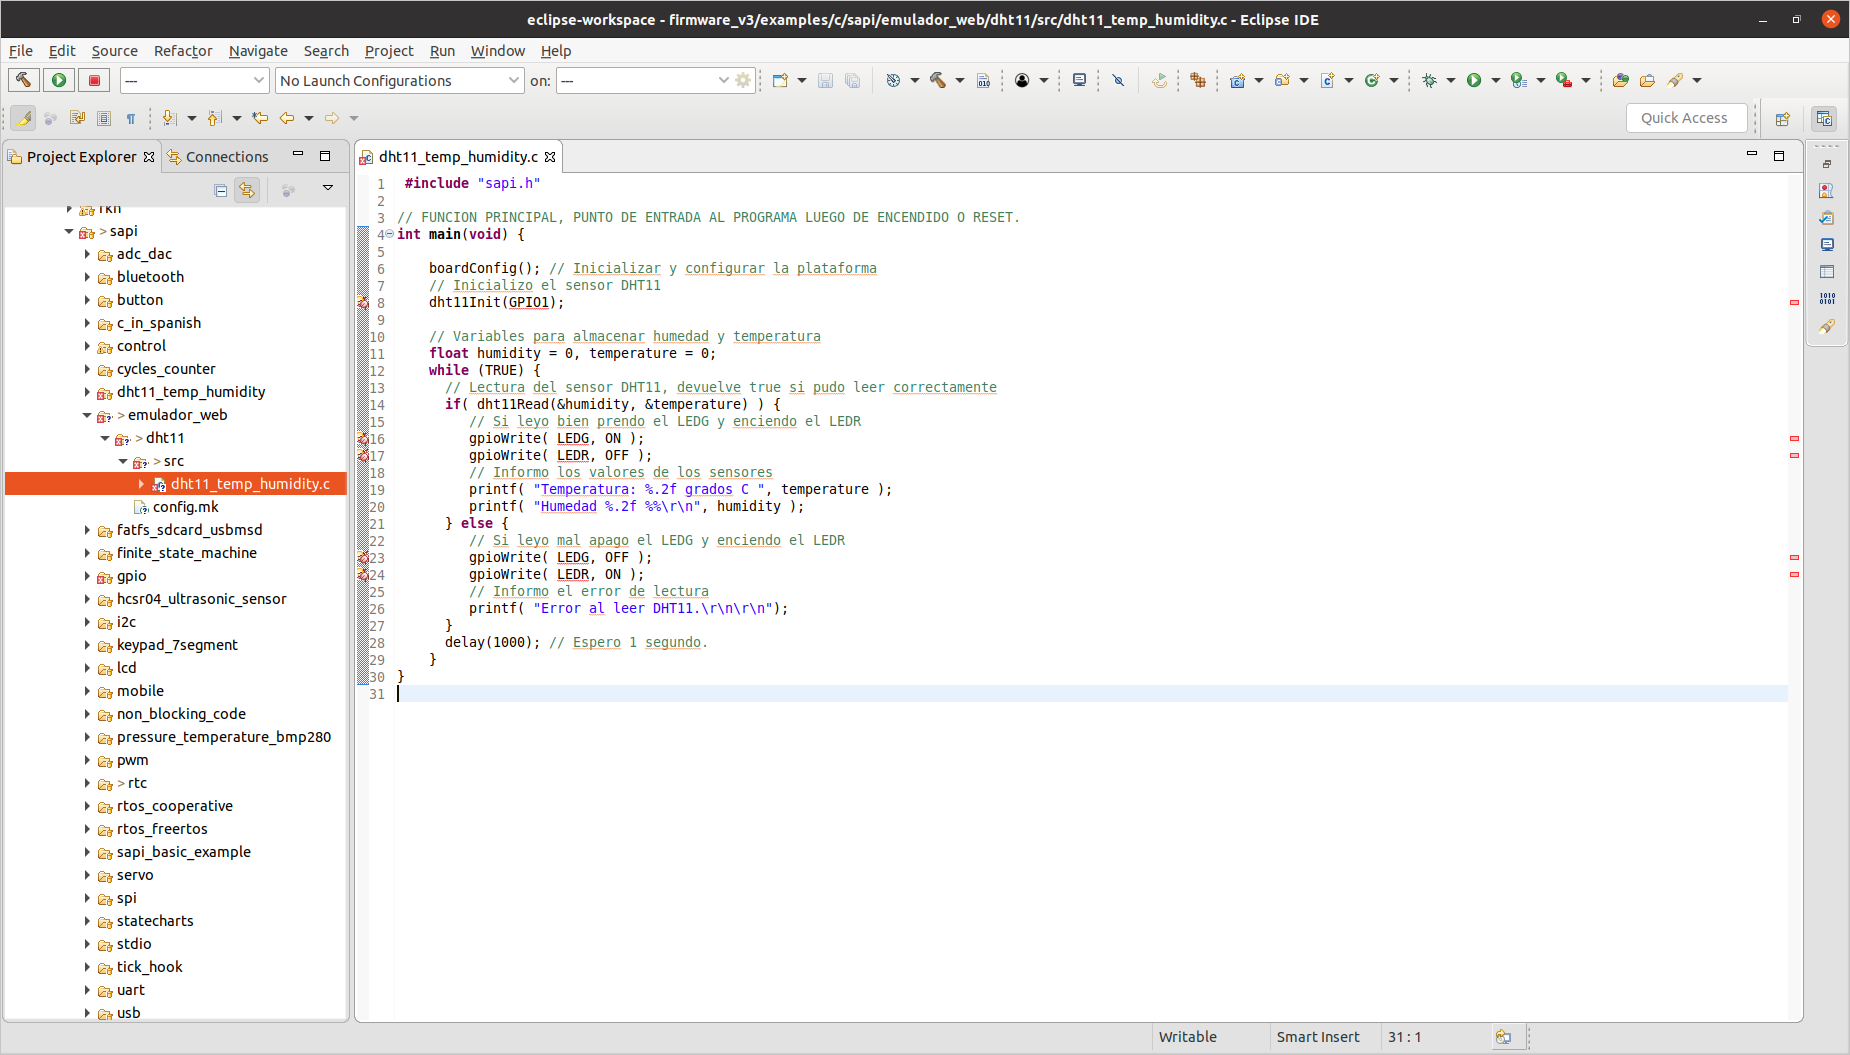
\includegraphics[scale=.20]{./Figures/TestEclipse.png}
	\caption{Código del ejemplo en eclipse.}
	\label{fig:TestEclipse}
\end{figure}

El programa \textit{\textbf{dht11}} de la plataforma de emulación es un ejemplo simple que solo enciende el LEDG en la placa y además, lee los datos generados del sensor DHT11 que consisten en temperatura/humedad. Luego, los datos leídos se imprimen por pantalla. 

En este ensayo manual, se registraron los cambios en la placa EDU-CIAA-NXP y también, los mensajes de la terminal serie. De modo que, posteriormente, permitió compararlos con la plataforma de emulación.

En la figura \ref{fig:TestPlaca} se observan los cambios en la placa EDU-CIAA-NXP que fueron registrados durante las pruebas.

\begin{figure}[ht]
	\centering
	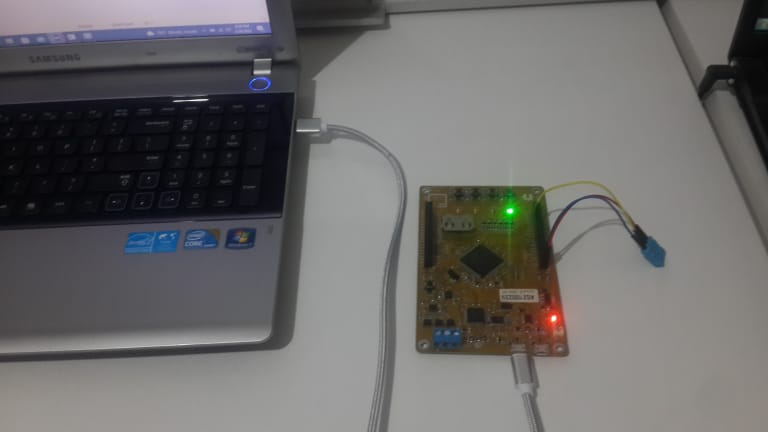
\includegraphics[scale=.50]{./Figures/TestPlaca.jpeg}
	\caption{Cambios en la placa EDU-CIAA-NXP durante el ensayo.}
	\label{fig:TestPlaca}
\end{figure}

Ahora bien, para leer los datos por pantalla se utilizó la herramienta \textit{Tera Term VT} que permitie guardar los datos de temperatura/humedad.

En la figura \ref{fig:TestTerminal} se muestra los datos de temperatura/humedad usando \textit{Tera Term VT}. 

\begin{figure}[ht]
	\centering
	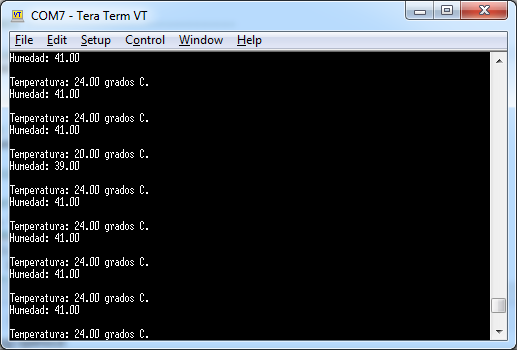
\includegraphics[scale=.90]{./Figures/TestTerminal.png}
	\caption{Salida de la terminal COM7, Tera Term VT.}
	\label{fig:TestTerminal}
\end{figure}

Resumen de la prueba Exitosa:
\begin{itemize}
	\item Después de acceder a la plataforma mediante el navegador y siguiendo los pasos del flujo principal y el flujo alternativo de la prueba, se comprobó que se muestra en ejecución el ejemplo \textit{\textbf{dht11}}.
	\item Se realizó la prueba de HTTP \textit{requests} usando la herramienta \textit{\textbf{Postman}} para comprobar la respuesta del \textit{\textbf{API openweathermap}} que consume la plataforma de emulación de manera que, los datos de temperatura y humedad sean los mismos.
	\item Se ensayo en la placa física EDU-CIAA-NXP  el mismo ejemplo \textit{\textbf{Dht11 temperature/humidity}} y se registraron los resultados de la terminal serial.
\end{itemize}

%----------------------------------------------------
\subsection{Prueba de creación de un nuevo proyecto, utilizando el código del ejemplo \textit{\textbf{tick\_hook}}}

El objetivo de este ensayo es exponer las diferencias en los resultados encontrados entre el emulador web y la placa física EDU-CIAA-NXP.

%--------------
\subsubsection{Ensayo en \textit{EmuCIAA}} 

Para ensayar la plataforma web, se ejecuta el siguiente caso de prueba:

\textit{\textbf{ID Caso de prueba: CP04}}

Descripción: la plataforma de emulación permite al usuario ejecutar el ejemplo \textit{\textbf{tick\_hook}} que se presenta en el código \ref{lst:codetickhook}.

\begin{lstlisting}[caption={Nuevo proyecto, basado en el ejemplo tick\_hook},label={lst:codetickhook},language=C]
#include "sapi.h"

void myTickHook( void *ptr )
{
   gpioWrite( LED3, ON );
   printf( "Blinky LED3.\r\n" );
   while(true) {
      printf( " while(true)  Blinky LED1.\r\n" );
      gpioToggle( LED1 );
      delay(1);
   }
}

int main()
{
    boardInit();
    tickInit(50);
    while(true) {
        tickCallbackSet( myTickHook, NULL );
        delay(5000);
    }
    return 0;
}
\end{lstlisting}

Pre-condición: 
\begin{itemize}
	\item La computadora del usuario tiene conexión a internet y un navegador web instalado.
\end{itemize}

Flujo principal:
\begin{enumerate}
	\item El usuario ingresa al entorno web \textit{EmuCIAA}.
	\item El usuario hace \textit{click} en el botón \textquotedbl Nuevo Proyecto\textquotedbl.
	\item La plataforma muestra al usuario en el área de codificacion, la pantalla para que pueda ingresar su propio codigo.
	\item El usuario ingresa el código de prueba \ref{lst:codetickhook}.
	\item El usuario hace \textit{click} en el botón \textquotedbl Ejecutar\textquotedbl.
	\item La plataforma muestra en la consola integrada la salida del programa en ejecución.
\end{enumerate}
	
La figura \ref{fig:Testtickhook} muestra en la consola integrada la salida de \textquotedbl Blinky LED3\textquotedbl muchas veces. 

\begin{figure}[ht]
	\centering
	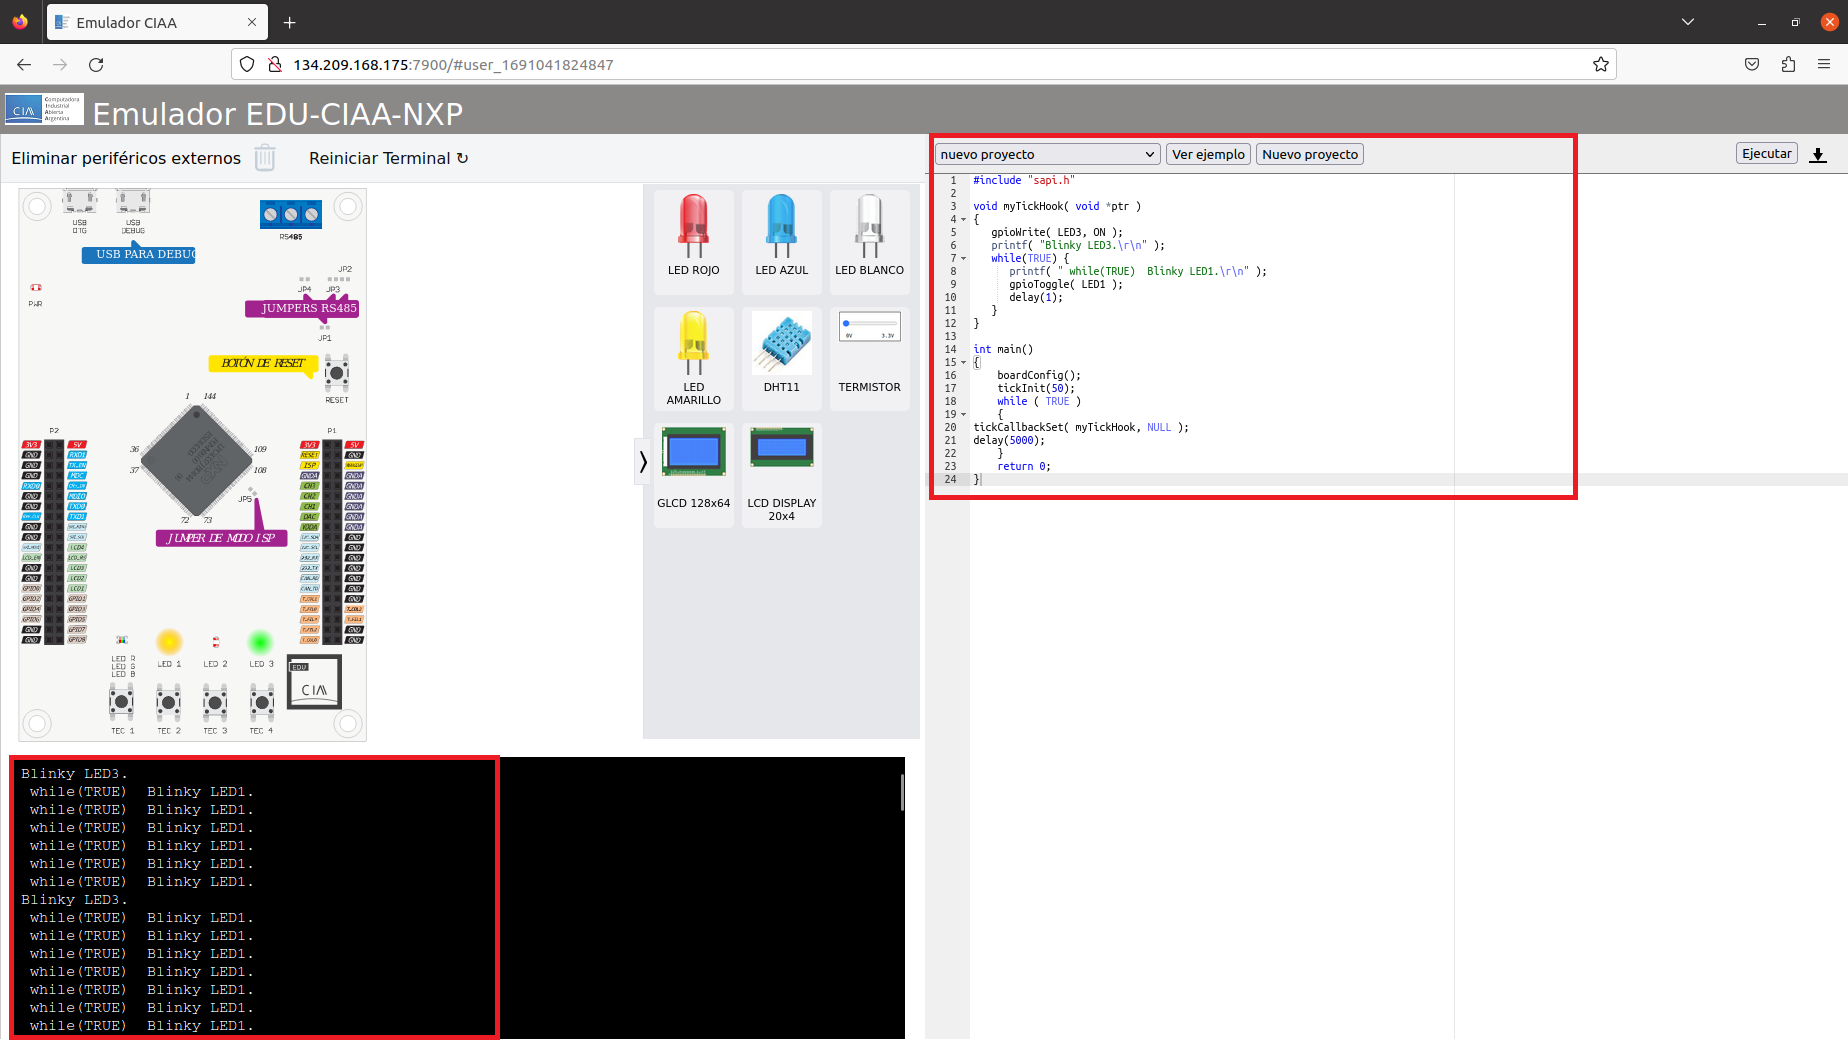
\includegraphics[scale=.20]{./Figures/Testtickhook.png}
	\caption{Salida por consola del ensayo tick hook.}
	\label{fig:Testtickhook}
\end{figure}

%----------------------
\subsubsection{Ensayo en la placa física EDU-CIAA-NXP} 

Se ejecuta el mismo ejemplo en la placa física EDU-CIAA-NXP y se obtiene por consola la siguiente salida que se muestra en la siguiente figura \ref{fig:TesttickhookPlaca}:

\begin{figure}[ht]
	\centering
	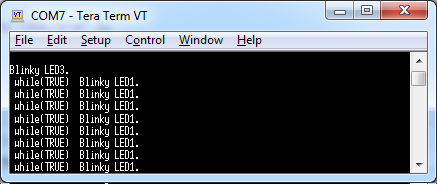
\includegraphics[scale=.80]{./Figures/TesttickhookPlaca.png}
	\caption{Salida de la terminal COM7 -Tera Term VT.}
	\label{fig:TesttickhookPlaca}
\end{figure}

Se observa que la salida por consola de \textquotedbl Blinky LED3\textquotedbl se muestra solo una vez, lo cual difiere de la salida por consola de la plataforma web que muestra \textquotedbl Blinky LED3\textquotedbl{} muchas veces.

La diferencia de este comportamiento en el emulador web esta relacionada con la forma en cómo JavaScript reanuda la ejecución después de que ocurre un tick. Por lo tanto, la forma en que se gestionan los estados en la ejecución de funciones puede diferir del comportamiento en la placa EDU-CIAA-NXP.

En un entorno físico, el sistema operativo o el microcontrolador pueden mantener un seguimiento del estado de la ejecución y reanudarla adecuadamente después de una interrupción de \textit{tick} del sistema. Sin embargo, para esta prueba en particular, dentro de la plataforma de emulación web, no se mantiene este estado de ejecución, lo que resulta en la repetición de ciertas porciones de código, como se ha demostrado.

Para solucionar esta diferencia en el entorno del emulador web, se podría explorar algunas opciones para mantener un seguimiento adecuado del estado de ejecución después de que ocurra un \textit{tick} del sistema. Este tema de manejo fino de tiempos y performance queda para trabajo a futro.

Se concluye entonces que para el uso en enseñanza de programación de Sistemas Embebidos la plataforma \textit{EmuCIAA} cumple con los requerimientos establecidos.